\section{Methods}
\vspace{-0.5cm}
\subsection{Nitrite Investigations}
\vspace{-0.5cm}
To obtain the voltammogram and calibration curves, DPV was performed on increasing concentrations of nitrite solution using the apparatus as described in figure X. The solution was degassed with nitrogen gas to remove oxygen impurities A 10$\%$ sulfamic acid solution was also added to reduce unreacted nitrite following completion.\\\\
A summary of performed experiments is shown below:

\begin{table}[H]
    \centering
    \begin{tabular}{ |p{3.7cm}||p{3.7cm}| } 
        \hline
        \multicolumn{2}{|l|}{\textbf{Reusable gold electrode}} \\ \hline
        Reusable gold electrode in PBS solution & Obtain baseline voltammetry and calibration curve for nitrite detection and estimate expected peaks\\ \hline
        Reusable gold electrode with 4\% albumin & Determine magnitude of effect of albumin in solution and compare to previous results \\ \hline
        \multicolumn{2}{|l|}{\textbf{Disposable gold electrode}} \\ \hline
    Disposable gold electrode in PBS solution & Obtain voltammetry and calibration curve and compare performance to reusable electrodes. \\ \hline
    Disposable gold electrode with 5.2 g/L albumin & Determine magnitude of effect of albumin in solution and compare to previous results\\ \hline
    \end{tabular}
    \label{tab:my_label}
\end{table}
Reusable gold electrodes were washed in an alumina polishing slurry prior to experimentation. Disposable electrodes were prepared by washing in 75\% ethanol, and the RE was coated with 5uM Polyhydroxyethylmethacrylate (pHEMA) and baked for one hour at 70\textdegree{C} \\
Detailed descriptions of performed experiments are listed in \autoref{app:nitrite_protocol}.


\begin{figure}[H]
\centering
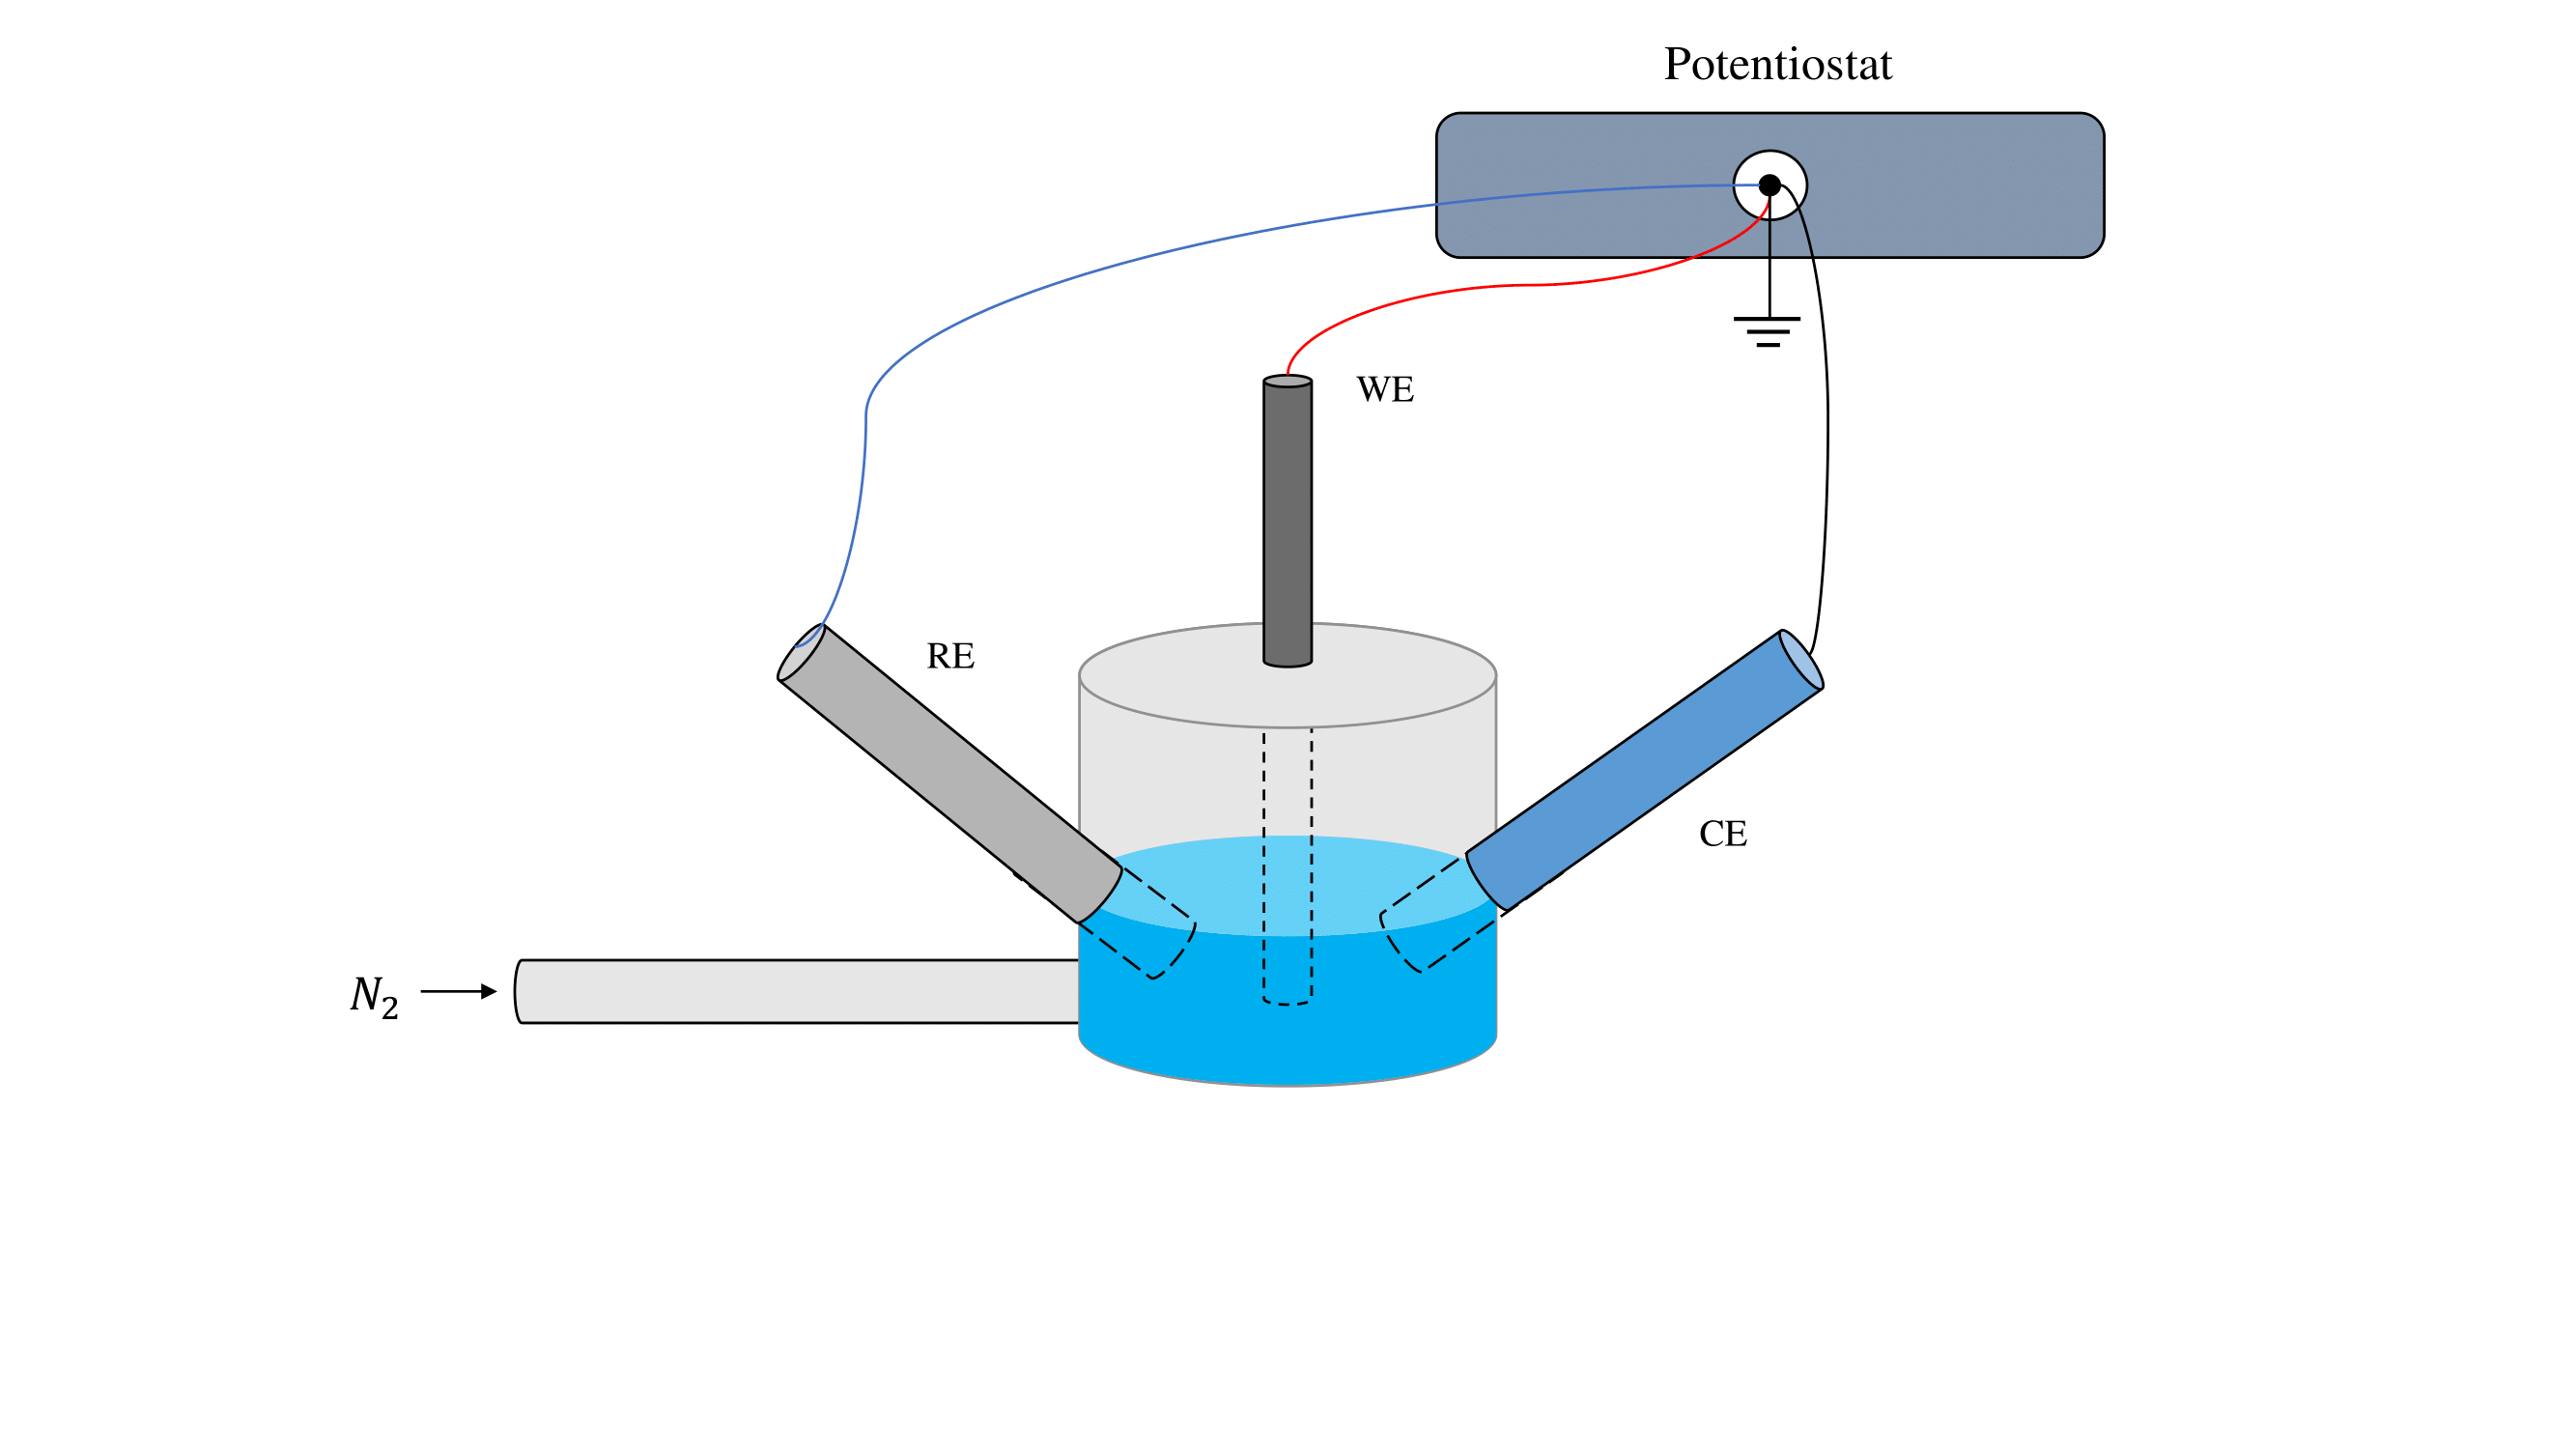
\includegraphics[width=0.5\textwidth]{img/james1.png}
\caption{Electrochemical cell schematic diagram: gold working electrode (WE), Ag/AgCl reference electrode (RE), platinum counter electrode (CE) in pH 7.4 phosphate-buffered saline (PBS). Measured using Palmsens Emstat$^3$}
\end{figure}

\begin{figure}[H]
\centering
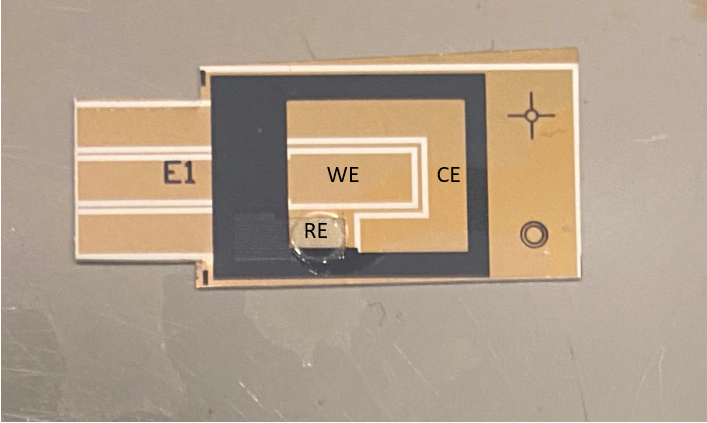
\includegraphics[width=0.45\textwidth]{img/disp electrode.PNG}
\caption{Image of gold disposable electrode. Working electrode (WE), Reference electrode (RE), Counter electrode (CE). pHEMA layer has been applied to RE.}
\end{figure}


\subsection{Hydrogen Peroxide Investigations}
To perform the sensing of hydrogen peroxide with Prussian blue, a four-step protocol has been established based on the publication by Chen \textit{et al} \cite{C9AN02438G}. Gold (Au) electrode were adopted for the calibration in the current stage. However, in our future work, disposable electrodes may be introduced for the blood sample testing. A detailed hydrogen peroxide electrochemical detection protocol can be found in \autoref{app:h2o2_protocol}. \\\\
The first step of the electrochemical detection involves the synthesis, crosslinking and coating of PEDOT: PSS-PB-EG-DVS complex. In this stage, 20\% v/v Ethylene glycol (EG) and 10\% v/v divinyl sulfone (DVS) have been added to the PEDOT:PSS-PB mixture to increase the mechanical stability of Prussian blue while maintain a high electrical conductivity. A gold working electrode coated with PEDOT: PSS-PB-EG-DVS complex is cured in oven at 110 \textsuperscript{$\circ$}C for 1 hour.
\begin{figure}[H]
    \centering
    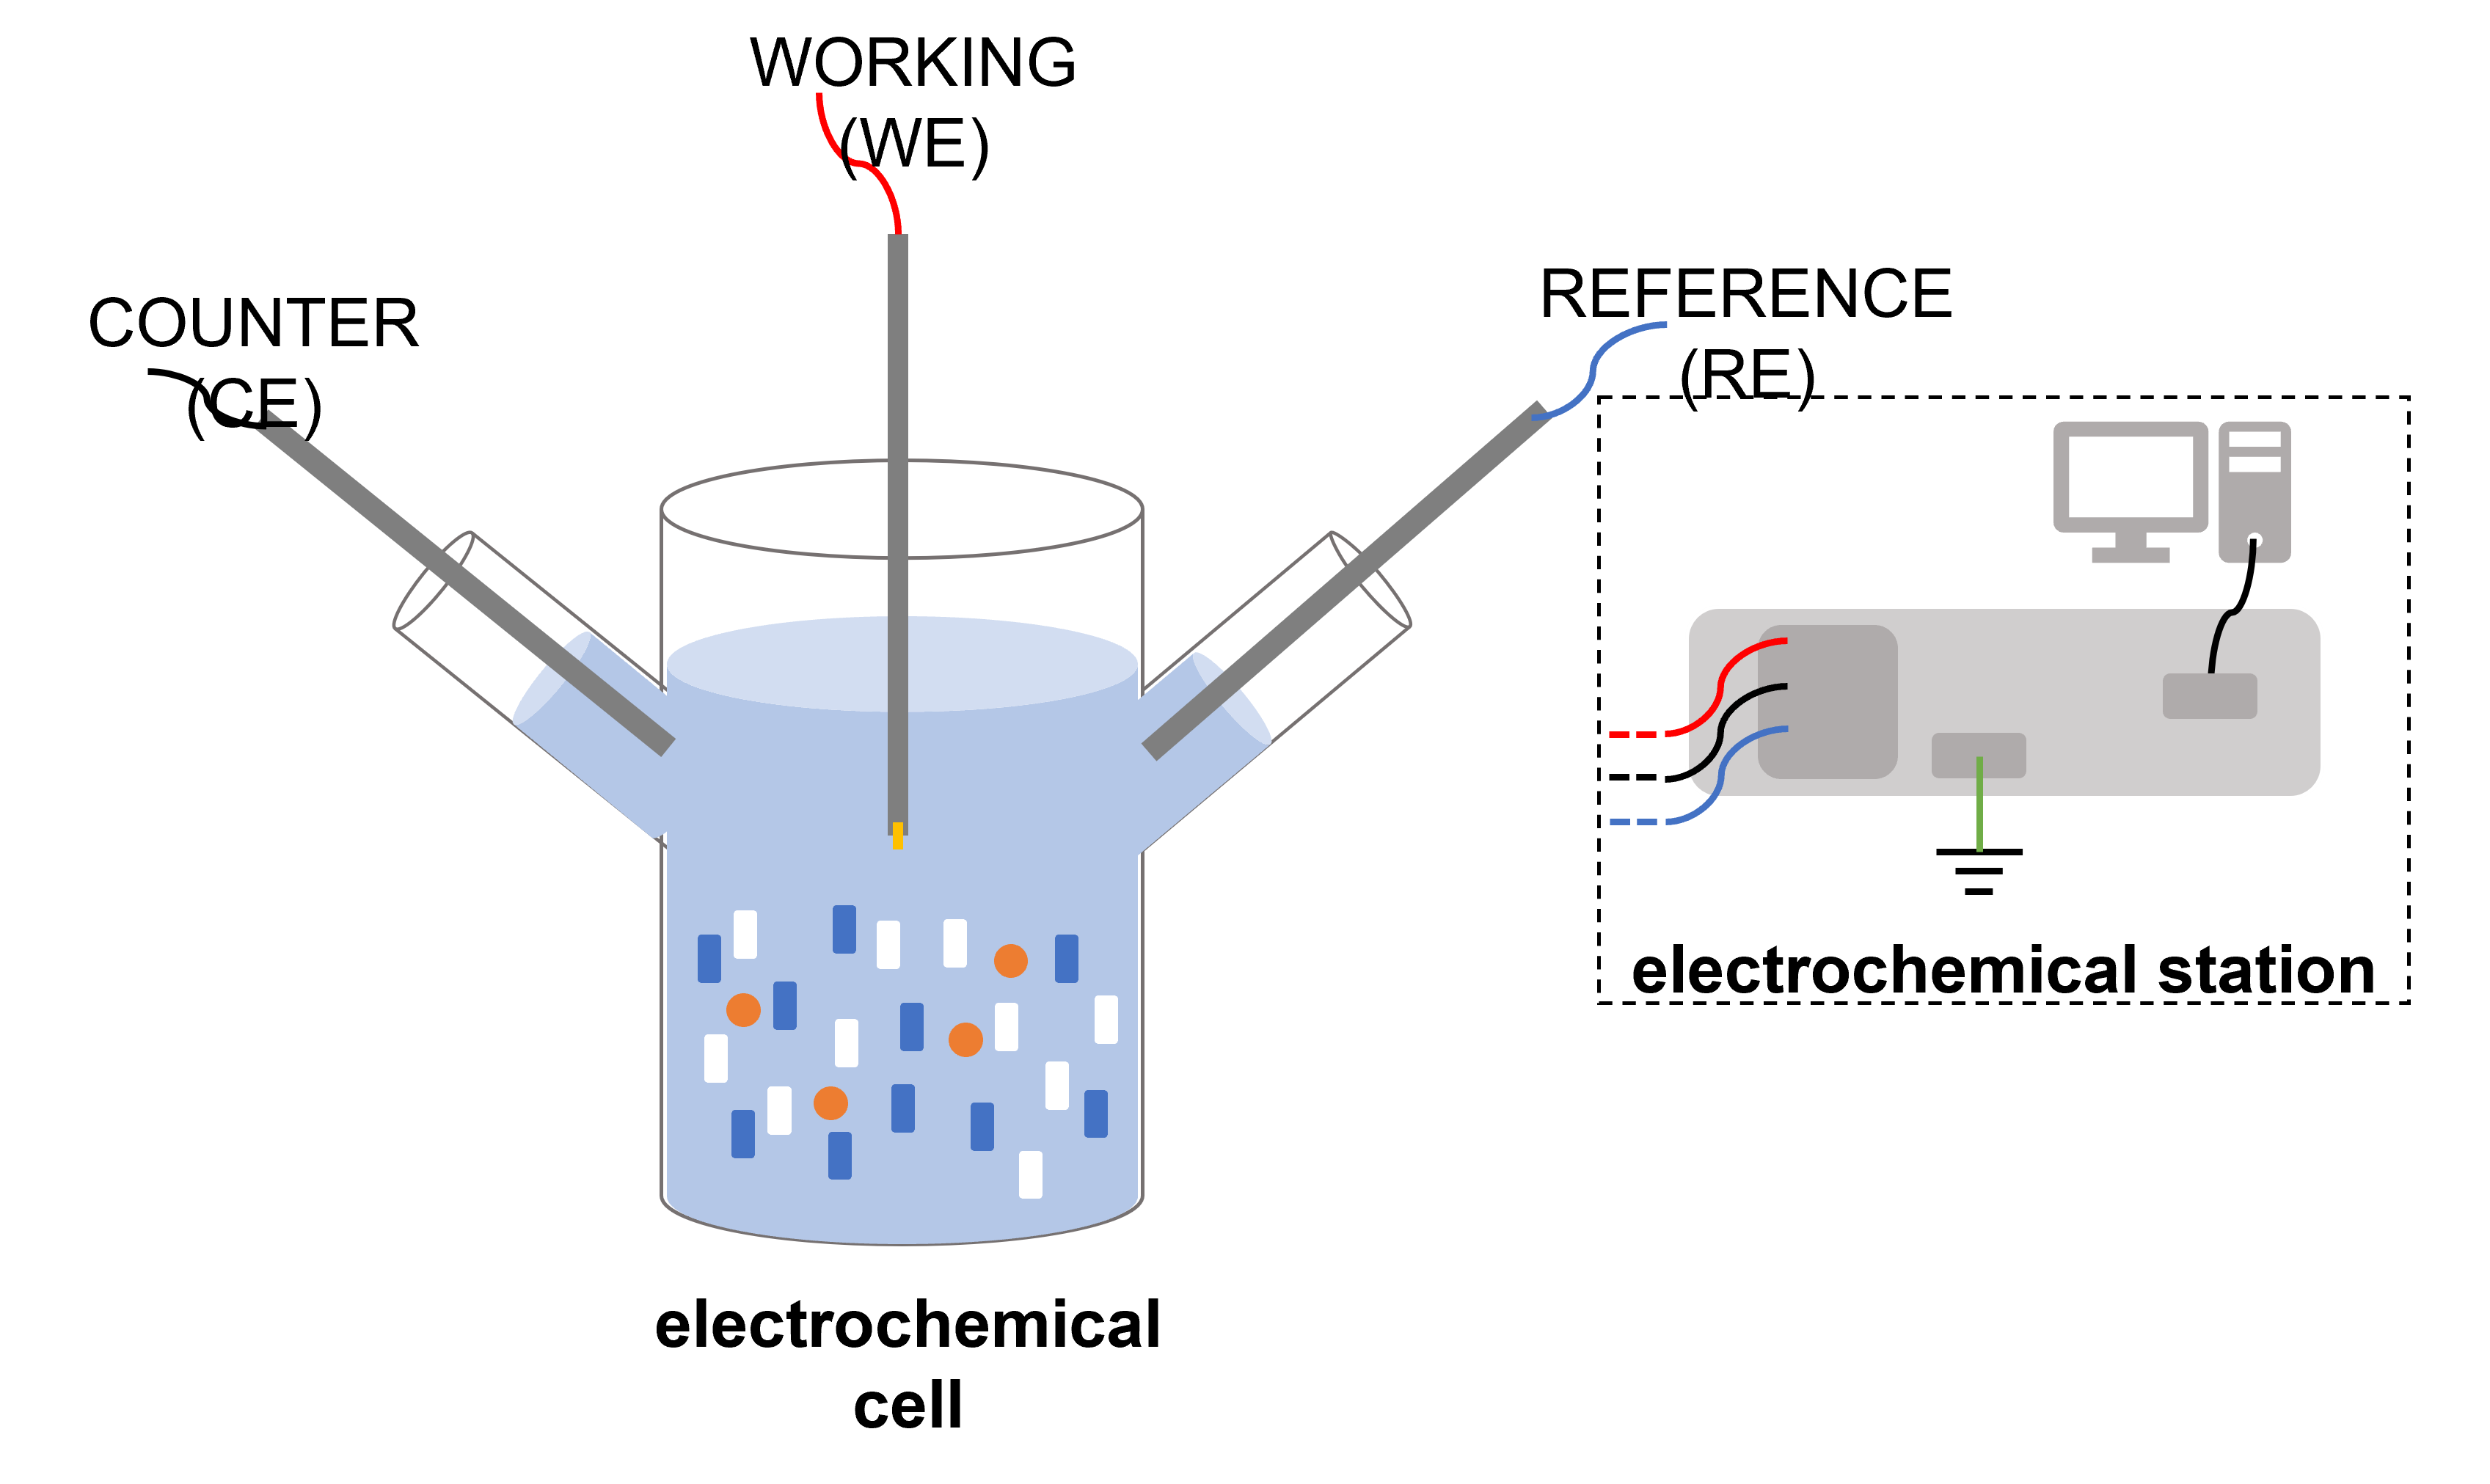
\includegraphics[width=.5\textwidth]{img/h2o2_setup.png}
    \caption{Hydrogen Peroxide experimental setup}
    \label{fig:h2o2_setup}
\end{figure}
\noindent The experimental setup for the hydrogen peroxide detection is shown in \autoref{fig:h2o2_setup}. With this setup, cyclic voltammetry was first performed in the blank buffer. This step is essentially a validation the existence of PB in the reaction environment. \\\\
\noindent Chrono amperometry was performed following the cyclic voltammetry scan. During this stage, a concentration range for hydrogen peroxide was set up from 50uM to 300uM. Hydrogen peroxide was added to the reaction environment gradationally to react with Prussian blue. Current and time data were collected under each concentration of hydrogen peroxide, coulometry was performed in the later stage for the experimental validation.

%====================================================================================
\subsection{Lactate Investigations}
Since lactate cannot directly engage in any redox reaction with the gold electrode, the sensor requires use of specific enzymes. Various enzymes, such as lactate oxidase (LOX) can be drop coated on to the surface of our electrode in a hydrogel matrix. The LOX can then oxidise lactate in the presence of oxygen to produce pyruvate and hydrogen peroxide. The peroxide can then be detected by the gold electrode.
\begin{align}
    Lactate + O_{2}  \xrightarrow{} Pyruvate + H_{2}O_{2}
\end{align}
\begin{align}
    H_{2}O_{2} + O_{2}  \xrightarrow{} 2e^{-}+2H^{+}
\end{align}
Various sensor fabrications can give rise to different sensitivity range. Ideally our sensor would to be able to detect lactate levels in the range of 0.5mmol/L to 4mmol/L, this would cover healthy and septic levels. The aim is to optimise detection range, this can be done by (i) selecting an enzyme with optimum kinetics (see appendix) or (ii)coating with Nafion membrane to reduce effect of interference \cite{rathee2016biosensors}. In this experiment electrodes were prepared using Nafion, a sulfonated fluoropolymer with a hydrophilic sulfonic component that can dissociate in solution, so the membrane is left negatively charged. This in turn, reduces the interference of anions in solution, therefore increasing specificity \cite{romero2010amperometric}. Electrodes were prepared from gold electrodes by coating with interference exclusion and enzyme hydrogel layers, see \autoref{app:lactate_protocol}.

The electrochemical cell was then set up using the lactate electrode as the working rotating disc electrode, platinum as the counter and Ag/AgCl as the working electrode with the following configuration: 

RDE is important for enzyme sensors as it maximises the proportion of mass transport due to convection and allows for a fully defined flow pattern around the electrode \cite{nikolic2000theoretical}. Amperometry was then conducted at 0.7V and 400rpm on 7.4pH PBS solutions spiked with 0.2mM/L aliquots in the 0.0-3mM/L range and then 0.5mM/L aliquots in the 3-4.5mM/L range. \subsection{Aptamer Modelling}
\subsubsection{Numerical Inverse Laplace Algorithm}
% Can put into the appendix if over word count
In chronoamperometric experiments on aptamer biosensors, the output signal is sampled at discrete time points. We therefore need to adapt the inverse laplace algorithm for discrete signals, by using a numerical linear least squares approach.\\\\
For a discrete signal we can use the numerical inverse Laplace transform to find the coefficients of the exponential decays (spectra G(k)).
The goal of the algorithm is to minimise the error between the model fit and the experimental data.
The discrete form of a general chronoamperometric signal can be represented as shown in \autoref{discretething}:
\begin{equation}
    y(t_{i}) = \sum_{j=1}^{N} \mathbf{G}(k_{j})e^{-t_{i}k_{j}}
    \label{discretething}
\end{equation}
where i is the index for the discrete time steps, and j is the index for the number of exponential decay components. In MATRIX form equation (\autoref{discretething}) can be represented as:
$$ \mathbf{y = AG} $$
where $ \mathbf{y}$ is a $M\times 1$ matrix, M is the number of time steps in the output current signal. $\mathbf{G}$ is a $N\times 1$ matrix, the coefficient for the exponential decay signals. $\mathbf{A}$ is a transfer matrix representing the kernel of the Laplace
transform, defined at every time point, with the rows of the matrix representing the time index and the columns of the matrix representing the number of exponential decay kernels (number of points in the computed decay rate distribution):$ [\mathbf{A}]_{ij} = e^{-k_{j}t_{i}} $, $y_{i} = y(t_{i}) $, $\mathbf{G}_{j} = \mathbf{G}(j)$.
We want to solve for $\mathbf{G}$, with the objective of minimising the error between the signal calculated using the model estimation of the output signal (AF) to the intrinsic experimental signal. This therefore becomes a linear least squares problem:\\\\
1D Ordinary linear least squares:
\begin{equation}
    min\lVert \mathbf{AG} - \mathbf{y}\lVert^{2}_{2}
\end{equation}
where $\mathbf{G}$ $\in$ $\mathbf{R}^{N}$.\\\\
The 'fminsearch' function in MATLAB is used to perform the minimization, using a derivative-free method to find the minimum of the unconstrained multivariable function.
As this problem of multiexponential decomposition is ill-posed and sensitive to noise, an additional regularizer must be added to constrain and smooth the output solution.
\begin{equation}
    V(\alpha) = \lVert \mathbf{AG} - \mathbf{y}\lVert^{2}+\alpha^{2}\lVert \mathbf{r} - \mathbf{RG}\lVert  = min
\end{equation}
$\mathbf{R}$ is a term that includes prior knowledge of the expected solution of $\mathbf{G}$. r is a matrix that represents the second derivative of $\mathbf{G}$. By taking the second derivative as the side constraint, we are effectively considering the curvature of G as a parameter to be minimised in the algorithm. The second derivative physically represents the rate of change of the gradient of the inverse laplace spectra $\mathbf{G(k)}$. Increasing the value of $\alpha$ therefore favors solutions which are smoother, as they have smaller values for the second derivative compared to noisy and spiky waveforms. See \autoref{app:apt_mod} for the code to perform these simulations.
\subsubsection{Coarse-grained Modelling of Aptamers}
To relate the electron transfer rates of the bound and unbound aptamer configurations ($k_{A}$, $k_{AT}$) to the distance the redox reporter (MB) is away from the electrode surface, we develop a model of aptamers in order to perform inverse modelling to predict the distribution of aptamer configurations.\\\\ 
Without considering chemical or thermodynamic effects of base-interactions within the Aptamer \cite{feigon1996aptamer}, we assume the aptamers to be a freely-jointed chain where the chains have the ability to rotate with 3DOFs.
The persistence length is a mechanical property quantifying the bending stiffness of a polymer. For double-stranded DNA (dsDNA), the persistence length has been widely reported as 50 nm \cite{bloomfielduniversity,marko1995stretching}. For single-stranded DNA (ssDNA), the short persistence length, fragile structure, and the appearance of stem loops complicates the measurement of persistence length. Latest measurements using atomic force microscopy shows a measurement of $1.98 \pm 0.72nm$ \cite{roth2018measuring}, in the range of previously published values of 1.5 - 3nm \cite{murphy2004probing,chi2013persistence}. For pieces of the ssDNA that are shorter than the persistence length, the molecule behaves like a rigid rod, while for pieces of the ssDNA that are much longer than the persistence length, the properties can only be described in a statistical fashion as a three-dimensional random walk.\\\\
For the aptamers we are testing in the laboratory, their base lengths range from 50 to 100, corresponding to base lengths of 17 and 34nm (length of single base = 0.34nm \cite{alberts2014molecular}), an order of magnitude larger than the persistence length of ssDNA. Therefore, in our model of Aptamers, we consider it as a freely-jointed chain with rigid segments of size $b = 2\zeta$ (where $\zeta$ is the persistence length). $b$ is also known as the Kuhn length \cite{strobl1997physics}.\\\\
In our model, we simulate random vectors in the spherical coordinate space for each of the rigid segments, and plot the end-to-end distance from the redox reporter (at the end of the ssDNA chain) to the electrode surface. In cases where any of the rigid segments reach below the electrode surface (z=0), we instead take the absolute z-value (maintain the randomly generated theta value, and recalculate the phi value such that the kuhn segment length is maintained), and continue the simulation. This therefore considers the redox reporter to bounce off the electrode in our random simulation model. 3D simulations for 100 bases (\autoref{Apt_sim}) in this freely-jointed chain model is shown, where we are interested in the end-to-end distance between the redox reporter and the electrode surface.\\\\
Extending the numerical simulation to 5E+06 simulations, the length distribution tends to a half gaussian, centred at the electrode surface (z=0). The width of the gaussian in principle depends on the length of the ssDNA chain (\autoref{L_dist}). 
\vspace{-3cm}
\begin{figure}[H]
    \centering
    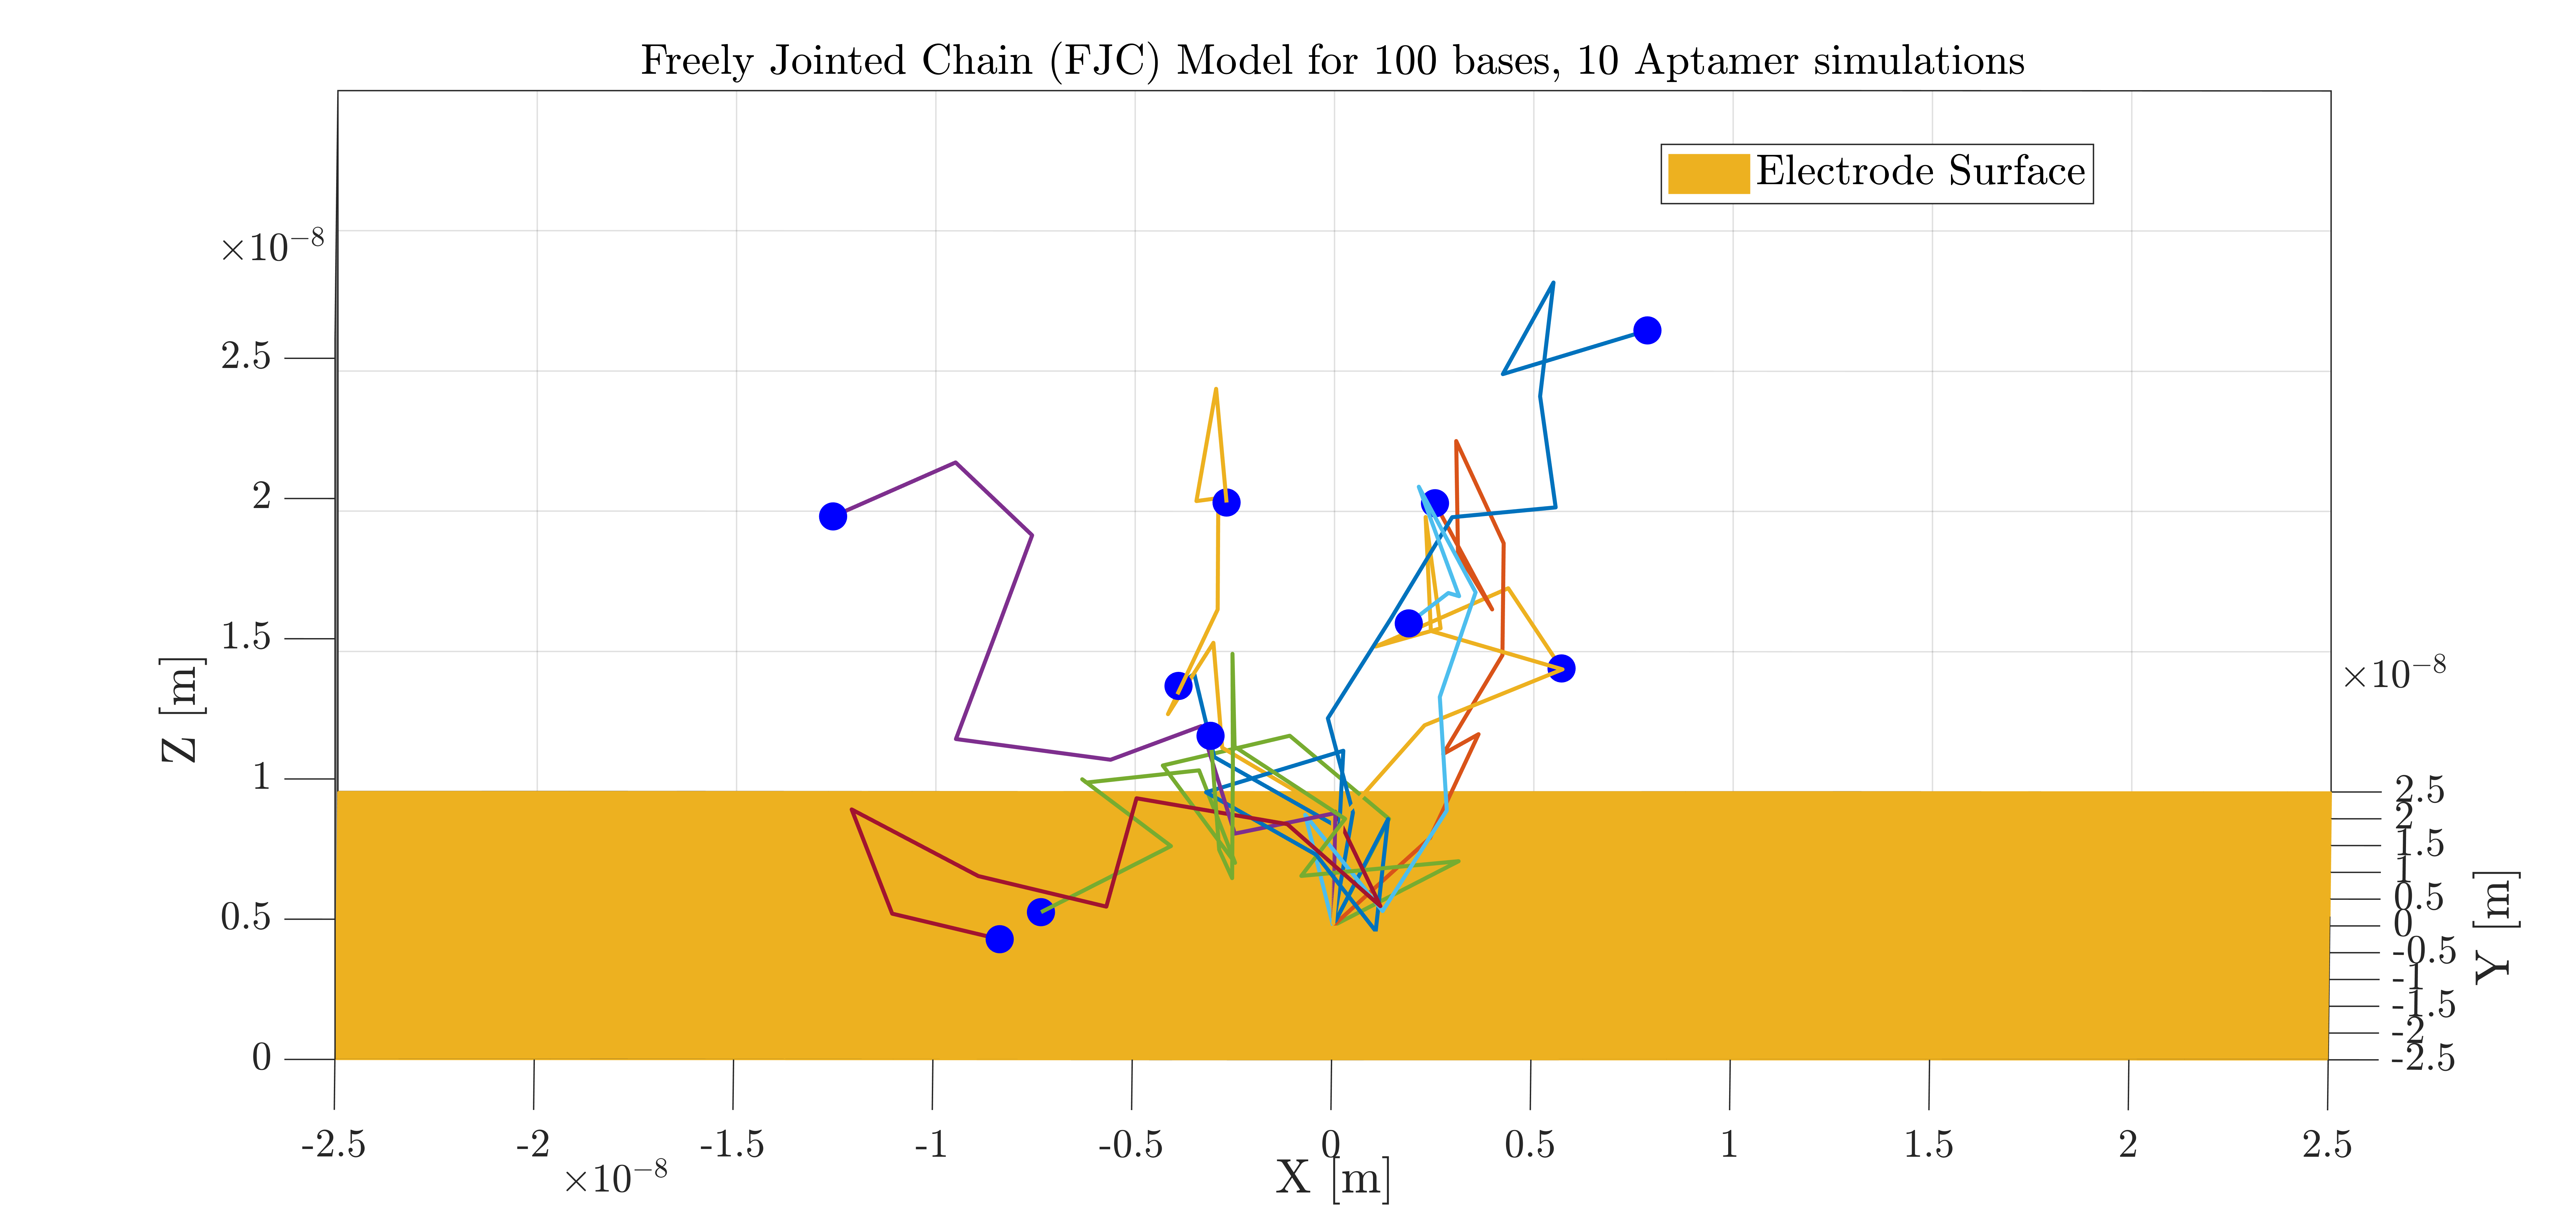
\includegraphics[width = 0.5\textwidth]{img/DNA_100_base_simulation_v1.png}
    \caption{Example plot of 10 Random Walk Simulations for 100 bases with Kuhn length segements (b = 2$\zeta$, where $\zeta$ is the persistence length of the DNA}
    \label{Apt_sim}
\end{figure}
\begin{figure}[H]
    \centering
    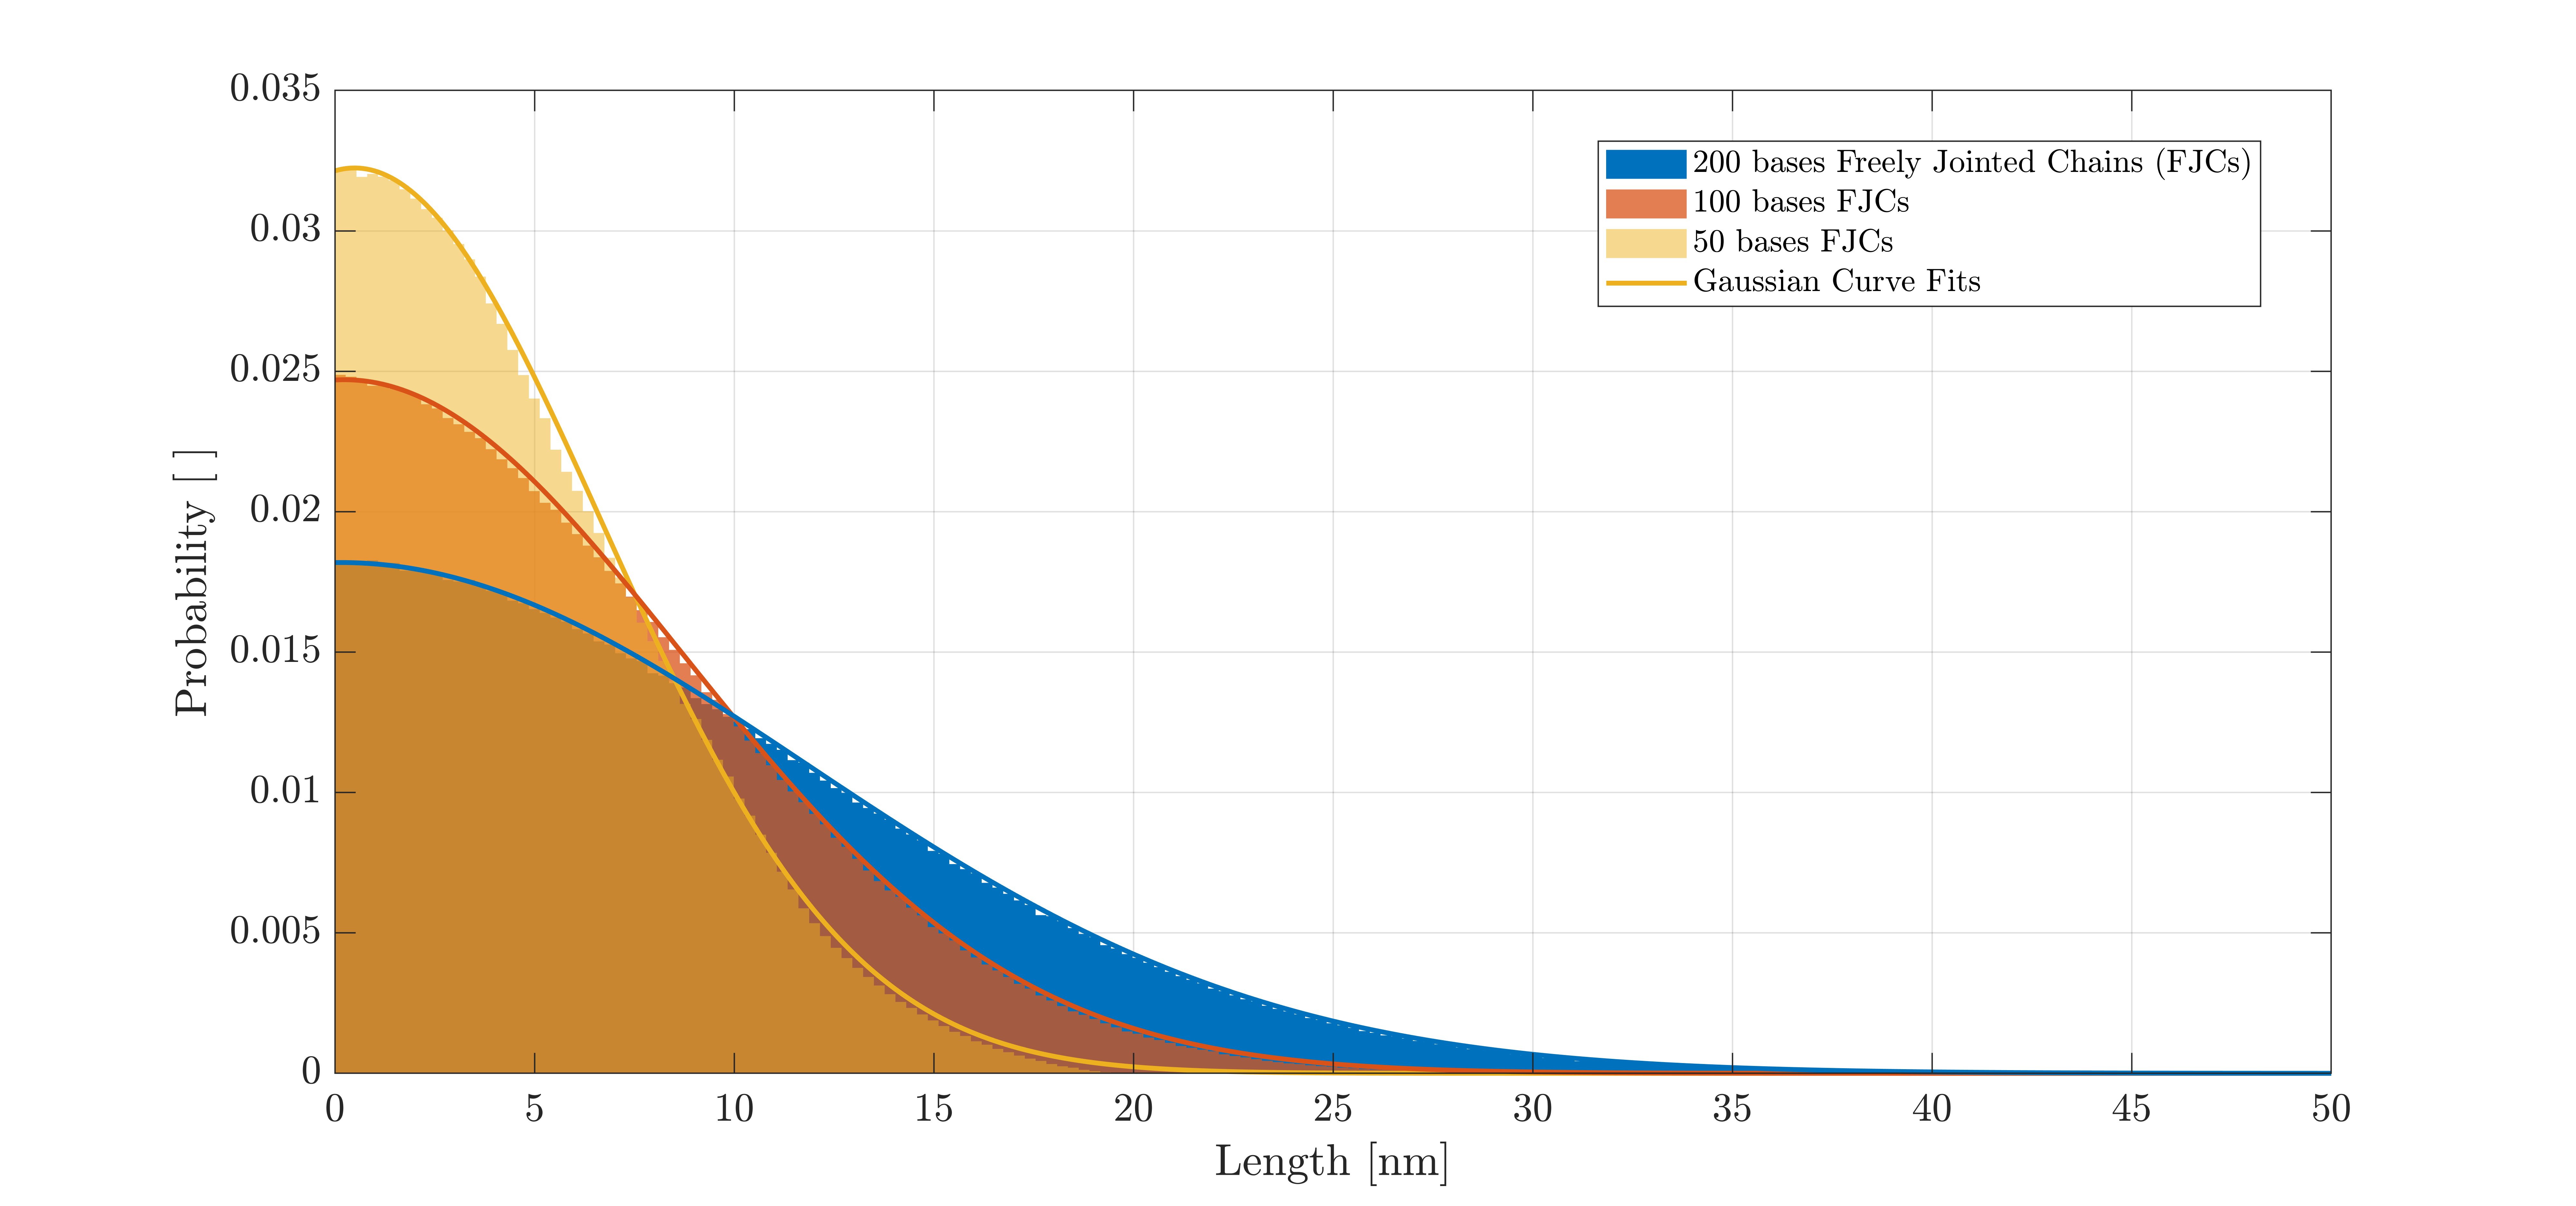
\includegraphics[width = 0.5\textwidth]{img/length_with_gaussians.png}
    \caption{Length probability distribution for Aptamers of 200, 100, and 50 base lengths. Numerically simulated using the freely-jointed chain model. Assume aptamer bounces off electrode surface when z$\leq$0. Probability distribution approaches a half-gaussian distribution. Gaussian fits overlayed, with parameters shown in table 1}
    \label{L_dist}
\end{figure}

